\documentclass[conference]{IEEEtran}
\usepackage[margin=1in]{geometry}
\usepackage{hyperref}
\usepackage{graphicx}
\usepackage{enumitem}
\usepackage{amsmath}
\usepackage{listings}
\usepackage{booktabs}
\usepackage{xcolor}
\usepackage{textcomp}
\usepackage{tikz}
\usetikzlibrary{calc, shapes.geometric, shapes.misc, arrows.meta, positioning}
\usepackage{tabularx}

\IEEEoverridecommandlockouts
% The preceding line is only needed to identify funding in the first footnote. If that is unneeded, please comment it out.
\usepackage{cite}
\usepackage{amsmath,amssymb,amsfonts}
\usepackage{algorithmic}
\usepackage{graphicx}

\def\BibTeX{{\rm B\kern-.05em{\sc i\kern-.025em b}\kern-.08em
    T\kern-.1667em\lower.7ex\hbox{E}\kern-.125emX}}

\lstdefinelanguage{Verus}{
    basicstyle=\ttfamily\footnotesize,
    keywords={type,let,match,case,of,if,then,else,print,as},
    keywords = [2]{Num,Str,Some,None},
    commentstyle=\color{gray},
    keywordstyle=\color{magenta},
    keywordstyle=[2]\color{blue},% for example
    numberstyle=\tiny\color{gray},
    stringstyle=\color{olive},
    basicstyle=\ttfamily\footnotesize,
    breakatwhitespace=false,         
    breaklines=true,                 
    captionpos=b,                    
    keepspaces=true,                 
    numbers=left,                    
    numbersep=2pt,                  
    showspaces=false,                
    showstringspaces=false,
    showtabs=false,                  
    tabsize=2,
    comment=[l]{//},
    commentstyle=\color{gray},
    morestring=[b]{"},
    sensitive=true
}

\begin{document}

\title{Verus: A Lambda Calculus Alternative to MISRA-C and CompCert\\
{\footnotesize https://github.com/adam-mcdaniel/verus}}

\author{\IEEEauthorblockN{1\textsuperscript{st} Adam McDaniel}
\IEEEauthorblockA{\textit{EECS Dept.} \\
\textit{University of Tennessee}\\
Knoxille, USA \\
amcdan23@vols.utk.edu}
\and
\IEEEauthorblockN{2\textsuperscript{nd} Alexander Krneta}
\IEEEauthorblockA{\textit{EECS Dept.} \\
\textit{University of Tennessee}\\
Knoxille, USA \\
akrneta@vols.utk.edu}
\and
\IEEEauthorblockN{3\textsuperscript{rd} Matthew Jones}
\IEEEauthorblockA{\textit{EECS Dept.} \\
\textit{University of Tennessee}\\
Knoxille, USA \\
mjone205@vols.utk.edu}
\and
\IEEEauthorblockN{4\textsuperscript{th} Kapildev Neupane}
\IEEEauthorblockA{\textit{EECS Dept.} \\
\textit{University of Tennessee}\\
Knoxille, USA \\
kneupan1@vols.utk.edu}
}

\maketitle

\begin{abstract}
Formally verified programming languages, such as MISRA-C and CompCert, play a crucial role in safety-critical systems by preventing classes of bugs that could result in catastrophic failures. However, these languages are based on C, which introduces unnecessary complexity and limitations due to its imperative and low-level nature. We introduce a new formally verified language based on the simply-typed lambda calculus, offering stronger static guarantees, improved expressiveness, and reduced developer burden. This project aims to show that such a language can outperform formally verified C while maintaining the same safety assurances and improving productivity.
\end{abstract}

\section{Introduction}
In recent years, due to many life-threatening software failures, such as the infamous Therac-25~\cite{therac25} radiation machine and the Boeing 737-MAX~\cite{boeing737max}, formally verified software has become a government-imposed mandate for devices in medicine, transportation, and aerospace. The vast majority of software written in these important industries uses formally verified languages based on C dialects, such as MISRA-C or CompCert ~\cite{boutekkouk2024}.

This C-based approach has an Achilles heel: the underlying language~C was designed for performance and flexibility, \emph{not} for static reasoning.  Pointer arithmetic, undefined behavior, and manual memory management combine to make proofs laborious and brittle. As a result, developer productivity is hindered --- developers are required to work harder to make their code pass the intense verification checks. Our hypothesis is simple: replace the C substrate rather than contort it.  By grounding a language in the Simply-Typed-Lambda-Calculus (STLC) --- where functions are total and side‑effects explicit --- many desirable guarantees emerge for free, enabling simpler tooling and lighter cognitive load for developers.

\section{Comparison With Existing Work}
There already exists a large ecosystem of verification‑oriented languages. On the functional-programming end of the spectrum, there's Agda, Coq, Idris and F\*, which wield dependent types to encode proofs alongside programs. On the more imperative-programming end of the spectrum, Rust introduces ownership to tame aliasing, and SPARK Ada strengthens Ada with contracts. However, none of these have become a suitable industry replacement for C because they~\cite{havelund2022}:

\begin{itemize}[nosep]
\item expose steep proof‑engineering overhead which introduces a significant cognitive load (Agda, Coq),
\item rely on heavyweight runtime infrastructure with fewer \emph{static} guarantees (Idris, Haskell), or
\item remain imperative at their core (SPARK Ada, Rust).
\item cannot provide certain guarantees, such as termination proofs (Rust).
\end{itemize}

Verus stakes out a middle ground: minimal calculus, eager termination, a more familiar C-like syntax compared to other functional languages, and the ability to extend the interpreter with well-checked built-in functions.

\section{Language Overview}

\subsection{Core Calculus}
Verus’s semantics are the Simply Typed Lambda Calculus augmented with sum, product, and list types, along with some other basic primitives:

\[
\begin{array}{c}
\tau = \textsf{Void}\;|\;\textsf{Bool}\;|\;\textsf{Str}\;|\;\textsf{Num}\;|\;
          [\tau_1]\;|\;
          \tau_1\times\tau_2\;\\|\;
          \tau_1+\tau_2\;|\;
          \tau_1\to\tau_2
\end{array}
\]

Below are the typing rules of STLC. These rules alone are needed to enforce the type-soundness of all expressions and guarantee termination of programs.

\[
\begin{array}{c}
\displaystyle
\frac{x:\sigma \in \Gamma}{\Gamma \;\vdash\; x:\sigma}
\quad (1)
\\\\\\
\displaystyle
\frac{c \text{ is a constant of type } T}{\Gamma \;\vdash\; c:T}
\quad (2)
\\\\\\
\displaystyle
\frac{\Gamma , x:\sigma \;\vdash\; e:\tau}
     {\Gamma \;\vdash\; (\lambda x:\sigma.\,e):(\sigma \to \tau)}
\quad (3)
\\\\\\
\displaystyle
\frac{\Gamma \;\vdash\; e_1 : \sigma \!\to\! \tau
      \quad
      \Gamma \;\vdash\; e_2 : \sigma}
     {\Gamma \;\vdash\; e_1\, e_2 : \tau}
\quad (4)
\end{array}
\]

Every program must be typable in this grammar; hence recursion must be \emph{structurally decreasing}, guaranteeing termination just like MISRA-C. This also means that Verus is not turing-complete, which makes \emph{many} more static proofs about memory, control flow, etc. tractable.

\begin{figure}[ht]
\centering
% ------------------------------------------------------------
%  Lambda cube with axis labels pulled farther from the figure
% ------------------------------------------------------------
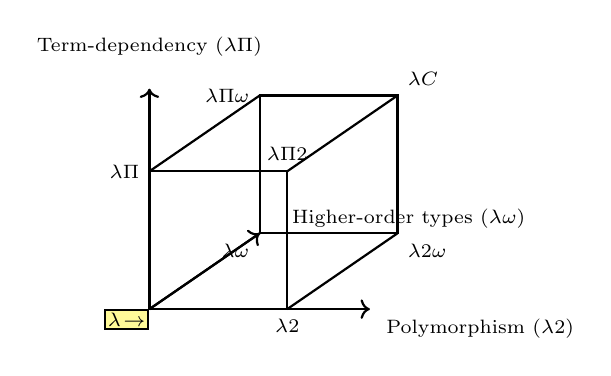
\begin{tikzpicture}[
        x=1.75cm, y=1.75cm,
        thick,
        every node/.style={font=\scriptsize}
]

%--- basis vectors (cabinet projection) ----------------------
\coordinate (O) at (0,0);            % origin
\coordinate (X) at (1.6,0);          % polymorphism axis
\coordinate (Y) at (0,1.6);          % term‑dependency axis
\coordinate (Z) at (0.80,0.55);      % higher‑order‑types axis

%--- axes with labels *beyond* the arrow tips ---------------
\draw[->] (O) -- (X)
      node[pos=1.5, below]  {Polymorphism ($\lambda 2$)};
\draw[->] (O) -- (Y)
      node[pos=1.1, left, anchor=south]
           {Term‑dependency ($\lambda\Pi$)};
\draw[->] (O) -- (Z)
      node[pos=1.2, right] {Higher‑order types ($\lambda\omega$)};

%--- front‑face vertices ------------------------------------
\coordinate (A) at (0,0);            % λ→   (STLC)
\coordinate (B) at (1,0);            % λ2
\coordinate (C) at (1,1);            % λΠ2
\coordinate (D) at (0,1);            % λΠ

%--- rear‑face vertices (front + Z) --------------------------
\coordinate (E) at ($(A)+(Z)$);      % λω
\coordinate (F) at ($(B)+(Z)$);      % λ2ω
\coordinate (G) at ($(C)+(Z)$);      % λC
\coordinate (H) at ($(D)+(Z)$);      % λΠω

%--- cube edges ----------------------------------------------
\draw (A)--(B)--(C)--(D)--cycle;     % front face
\draw (E)--(F)--(G)--(H)--cycle;     % rear face
\draw (A)--(E) (B)--(F) (C)--(G) (D)--(H);

%--- vertex labels -------------------------------------------
\node[draw, fill=yellow!40, inner sep=1pt] at (A) [below left] {$\lambda\!\to$};
\node at (B) [below]      {$\lambda 2$};
\node at (D) [left]       {$\lambda\Pi$};
\node at (C) [above]      {$\lambda\Pi 2$};

\node at (E) [below left] {$\lambda\omega$};
\node at (F) [below right]{$\lambda 2\omega$};
\node at (H) [left]       {$\lambda\Pi\omega$};
\node at (G) [above right]{$\lambda C$};

\end{tikzpicture}
\caption{Depiction of Barendregt's Lambda Cube, with Simply Typed Lambda Calculus's coordinates highlighted in yellow.}
\label{fig:verus-pipeline}
\end{figure}

This type system lies squarely at the origin of Barendregt's Lambda Cube, while most other functional-oriented verification languages lie in the upper face of the cube\cite{barendregt1991}.

\subsection{Surface Syntax}
Adopting braces, semicolons and \texttt{let} bindings keeps the learning curve low for C engineers while preserving functional purity.

\paragraph{Enumerations and pattern matching.}
\begin{lstlisting}[language=Verus, caption={Safe integer division with algebraic data types.}, numbers=left]
{
    // Create a union/sum type that can represent a number, or void.
    type MaybeNum = {Some(Num) | None};

    // Create a division function that
    // returns None for an undefined result,
    // or Some number otherwise.
    let div n: Num, d: Num =
        // If the denominator is zero,
        // return None.
        if d == 0 then MaybeNum of None
        // Otherwise, return Some result.
        else MaybeNum of Some (n / d);

    // A function that tests the division
    // result.
    let test_div n: Num, d: Num =
        // Use pattern matching
        // on the division result:
        match div n d with
            // If the result is some number,
            // print the equation result.
            case of Some(result) =>
                print (n as Str)
                    & " / "
                    & (d as Str)
                    & " = "
                    & (result as Str),
            // If there's no number, print that
            // the division is undefined.
            case of None =>
                print (n as Str)
                    & " / "
                    & (d as Str)
                    & " is undefined";

    // Test the divion of 10/2
    test_div 10 2;
    // Test the division of 10/0
    test_div 10 0;
}
\end{lstlisting}

\paragraph{First‑class higher‑order functions.}

\begin{lstlisting}[language=Verus, caption={Total factorial using range/product combinators}, numbers=left]
{
    // Create a lambda function and bind
    // it to the name `factorial`
    let factorial =
        \n: Num -> product (range 1 n + 1);

    // Get the first command-line argument,
    // after the executable path,
    // and check whether it exists.
    match (args ())@1 with
        // If it exists, calculate the
        // factorial of the passed number
        case of Some(x) => {
            let n = x as Num;
            // Print the result.
            print "Factorial of "
                  & (n as Str)
                  & " is "
                  & ((factorial n) as Str);
        },
        // If it doesn't exist,
        // print an error message.
        case of None =>
            print "Please provide a number.";
}
\end{lstlisting}

\paragraph{Structures and member-accesses.}
\begin{lstlisting}[language=Verus, caption={Point structure and manipulation with functions.}, numbers=left]
{
    // Declare a 2D point structure.
    type Point = {
        // The X component of the point.
        x: Num,
        // The Y component of the point.
        y: Num
    };

    // A function that shifts a point
    // by a delta-x and delta-y component.
    let move p:Point, dx:Num, dy:Num =
        {x: p@x + dx, y: p@y + dy};
        
    // Force the variable `p` to be declared
    // as a Point type by the type-checker.
    let p: Point = {x: 5, y: 6};

    // Shift `p` by 1 and 2 in the X and Y
    // components respectively.
    // 
    // Use type inference to declare `p2`
    // as a point.
    let p2 = move p 1 2;

    // Print the shifted point.
    print p2;
}   
\end{lstlisting}

\subsection{Safety Guarantees}
STLC provides many critical properties \emph{by construction} --- these are guarantees resulting from the structure of the type-system alone:

\begin{itemize}[nosep]
\item \textbf{Progress} (no stuck terms): A well‑typed expression is either a value or can make progress towards the final resulting expression. In other words, every well-typed program has a possible evaluation step remaining or the program is a constant value.
\item \textbf{Preservation}: Evaluation preserves types. This helps prevent undefined behavior and induction to be applied heavily to infer most types in programs.
\item \textbf{Strong normalization}: All reduction sequences terminate.
\end{itemize}

Because of the strong normalization property of STLC, as proven by Tait in 1967, memory safety checks and the proven absence of undefined behavior are possible without the near 200 aditional MISRA-C safety rules~\cite{tait1967}.

\section{Evaluation Strategy}

\tikzset{
  doc/.style    ={draw, shape=document, minimum width=2.0cm,
                  minimum height=1.2cm},
  cyl/.style    ={draw, shape=cylinder, aspect=0.3, minimum width=2.2cm,
                  minimum height=1.4cm},
  banner/.style ={draw, rectangle, rounded corners=1pt, fill=yellow!40,
                  minimum width=3cm, minimum height=1cm},
  error/.style  ={draw, star, star points=9, fill=red!70,
                  minimum size=1.3cm},
  ->, >=Latex, thick
}
% ------------------------------------------------------------------

\begin{figure}[ht]
\centering
\begin{tikzpicture}[font=\small]

%-------------------------------------------------
\node[doc]                       (input) {Input program};

\node[cyl,  below=of input]      (ast)   {AST};

\node[cyl,  below=of ast]        (vast)  {Statically Verified AST};

\node[rectangle, draw, rounded corners=2pt,
      below=of vast]             (interp){Interpreter};

\node[banner, below=of interp]   (output){Output};

\node[error, right=1.8cm of ast] (err)   {Error};

%-------------------------------------------------
\draw (input)  -- node[right]{\textbf{Parser}}       (ast);
\draw (ast)    -- node[right]{\textbf{Type Checker}} (vast);

\draw (ast) -- ++(0.8,0) |- (err);

\draw (vast)  -> (interp);
\draw (interp)-> (output);

\end{tikzpicture}
\caption{Flow diagram of Verus's verification and execution.}
\label{fig:verus-pipeline}
\end{figure}
% ------------------------------------------------------------------
\subsection{Front‑End}
A recursive-descent parser built with \texttt{nom} produces an abstract syntax tree (AST). The type‑checker is a direct transcription of the STLC rules. If the syntax of the input program is invalid, the program is rejected and is not pipelined through the other evaluation steps.

\subsection{Type-Checker}

If the parser returns a valid AST, then it is passed through the type-checker to verify the input program. The type-checker infers types which are not listed, and confirms that no mismatched types exist in the program. This includes confirming the validity of function applications, variable assignments, and member accesses of structures, and the indexing of list elements.

\subsection{Back‑End}
Instead of emitting assembly, Verus uses a minimal interpreter to evaluate the code. A compiler could be built for Verus, but that is beyond the scope of this work. The interpreter receives an expression and an evaluation environment in which to interpret the expression. The initial environment is populated with standard library built-in functions. Lambda functions close over the environment they're evaluated in --- they collect the variables from their parent scope and add them to their own scope when they're called later on.

\subsection{Runtime Model}
\begin{itemize}[nosep]
\item \textbf{Functions}: Functions are stored as closures which capture symbols used in their function body from the parent environment.
\item \textbf{Heap}: While heap usage is not restricted, calculating the maximum heap usage during runtime is decidable given that STLC is strongly normalizing. So, memory usage can be restricted in practice similar to MISRA-C.
\item \textbf{Interpreter}: Verus is implemented with an interpreter in place of a compiler. This was done for simplicity and the sake of time --- a compiler would be more desirable.
\end{itemize}

\section{Rationale: Why STLC Over C?}

\paragraph{Simpler proofs}
Soundness of STLC fits on a whiteboard~\cite{pierce2002}; CompCert's proof spans \(\sim\)120,000 lines of Coq~\cite{leroy2006}, for example.  Verus transfers proof obligations from each program to the \emph{language design} -- no control-flow annotations are required.

\paragraph{Fewer developer constraints}
MISRA-C has many restrictions on user-code that are lifted in a STLC-based approach. For example, sum-types (\verb|union| in C) are disallowed in MISRA-C~\cite{MISRA2004}, while our STLC-based approach allows for statically checked sum-types with pattern matching.

\paragraph{Expressive abstractions}
Algebraic data types, pattern matching, and higher order functions increase developer productivity by allowing more flexibly written code~\cite{hughes1989}. These features are built into the type system in Verus, while C can only provide similar code structure with macros. 

\paragraph{Deterministic execution}
Because all functions terminate and the side effects are explicit, the analysis of the worst-case execution time is tractable. This is highly desirable for mission-critical applications.

\section{Trade‑Offs and Open Challenges}
\begin{enumerate}[label=\roman*., nosep]
\item \textbf{Mutable state.}  Pure lambda-calculus forbids mutation~\cite{barendregt1984}; embedded software often demands it\cite{vahid2002}. However, compiler optimizations, such as those implemented for languages like Haskell, can be effective in making functional-style code just as performant as imperative code~\cite{burn1988}.
\item \textbf{Low‑level bit‑tricks.}  Cryptographic software in C relies on "bit‑twiddling"~\cite{warren2002}.  A \texttt{Bits} primitive may be introduced with verified semantics, but this was not implemented in this work.
\item \textbf{Ecosystem inertia.}  Tooling, linters and IDE integrations must reach parity with current C workflows to gain traction. This is unlikely given the inertia behind C.
\item \textbf{The Verus Interpreter.} Most formally verified software is designed for use on embedded devices. The Verus interpreter is not desirable for these use-cases --- a compiler must be implemented to effectively address this. This could be done by modifying existing functional language compilers.
\end{enumerate}

\section{Possible Future Work}
\begin{enumerate}[label=\arabic*., nosep]
\item \textbf{A Verus compiler.} Transitioning to compilation instead of interpretation would certainly make Verus a more attractive option for typical industry applications. It would also significantly boost runtime performance.
\item \textbf{A larger standard library.} More built-in functions and types in the standard library could drastically improve developer productivity by reducing the amount of user-code required to achieve common operations and abstractions.
\item \textbf{The addition of memory usage analysis.} Although statically proving the required memory for programs is desirable and tractable in Verus's language model, it is not currently implemented in this work. Future work could expand on the current infrastructure to include this in the type-checker.
\end{enumerate}

\section{Conclusion}
This work demonstrates that a Simply Typed Lambda Calculus provides a compelling foundation for formally verified programming languages in safety-critical domains. By implementing a prototype STLC-based language with a more C-like syntax, we have shown a fundamentally different approach to formal verification than MISRA-C and CompCert. While traditional approaches take a Turing-complete language (C) and impose restrictions to make it safe~\cite{seacord2005}, our approach begins with an inherently safe, non-Turing-complete foundation and carefully adds features to increase expressiveness without compromising safety guarantees.

STLC programs are guaranteed to terminate by construction, eliminating the need for control flow annotations to explicitly prove termination. Potentially accelerating development cycles while maintaining reliability standards for industries where formal verification is mandated. Our implementation demonstrates that STLC-based languages allow for many language features that are impossible in C-based approaches, such as algebraic data types, pattern matching, and higher-order functions, all while maintaining stronger static guarantees.

Verus demonstrates the potential for improving the developer experience in formally verified systems without sacrificing safety. While this prototype serves as a proof-of-concept, future STLC-based would need polished compilation capabilities, memory analysis tools, and expanded libraries to be viable alternatives in industry settings. Our results suggest that lambda calculus offers a promising path forward for critical systems development--one that balances rigor with practicality and reduces the burden currently imposed by C-based verification frameworks.
\bibliographystyle{plain}
\begin{thebibliography}{9}
% \bibitem{misra}
% MISRA C Working Group, \emph{MISRA‑C:2012 Guidelines for the Use of the C Language in Critical Systems}.
% \bibitem{compcert}
% X.~Leroy, \emph{Formal Verification of a Realistic Compiler}.
% \bibitem{stlc}
% H.~Barendregt, \emph{The Lambda Calculus: Its Syntax and Semantics}.

\bibitem{therac25}
A.~Fabio, ``Killed by a Machine: The Therac-25,'' \emph{Hackaday}, Oct. 26, 2015. [Online]. Available: \url{https://hackaday.com/2015/10/26/killed-by-a-machine-the-therac-25/}. [Accessed: May 7, 2025].

\bibitem{boeing737max}
G.~Travis, ``How the Boeing 737 Max Disaster Looks to a Software Developer,'' \emph{IEEE Spectrum}, Apr. 18, 2019. [Online]. Available: \url{https://spectrum.ieee.org/how-the-boeing-737-max-disaster-looks-to-a-software-developer}. [Accessed: May 7, 2025].

\bibitem{boutekkouk2024}
F. Boutekkouk, E. Bouaghi, and O. Bouaghi, “C Software Formal Verification Review, Challenges and Future Directions,” in *Proceedings of the 2024 IEEE International Conference on Software Engineering and Formal Methods (SEFM 2024), Sep. 2024, pp. 1–8.

\bibitem{havelund2022}
K.~Havelund, “A Half Century of Formal Methods—Challenges and Trends,” in \emph{Proc. FM-50 Workshop}, Lecture Notes in Computer Science, vol. 13448, 2022. [Online]. Available: \url{https://www.havelund.com/Publications/fm-50-2022.pdf}. [Accessed: May 7, 2025].

\bibitem{tait1967}
W.~W. Tait, “Intensional interpretations of functionals of finite type I,” \emph{J. Symbolic Logic}, vol.~32, no.~2, pp. 198–212, Aug. 1967.

\bibitem{pierce2002}
B.~C. Pierce, \emph{Types and Programming Languages}. Cambridge, MA, USA: MIT Press, 2002.

\bibitem{leroy2006}
X.~Leroy, “Formal certification of a compiler back-end or: Programming a compiler with a proof assistant,” in \emph{Proc. 33rd ACM SIGPLAN-SIGACT Symp. Principles of Programming Languages (POPL)}, Salt Lake City, UT, USA, Jan. 2006, pp. 42–54.

\bibitem{MISRA2004}
Motor Industry Software Reliability Association, \emph{MISRA-C:2004 — Guidelines for the use of the C language in critical systems}, Coventry, UK: MISRA, Oct. 2004.

\bibitem{hughes1989}
J.~Hughes, “Why functional programming matters,” \emph{The Computer Journal}, vol.~32, no.~2, pp. 98–107, Apr. 1989. DOI: 10.1093/comjnl/32.2.98.

\bibitem{barendregt1984}
H.~P. Barendregt, \emph{The Lambda Calculus: Its Syntax and Semantics}, 2nd ed. Amsterdam, The Netherlands: North-Holland, 1984.

\bibitem{vahid2002}
A.~Vahid and T.~Givargis, \emph{Embedded Systems: A Contemporary Design Tool}. San Francisco, CA, USA: Morgan Kaufmann, 2002.

\bibitem{burn1988}
G.~L. Burn, S.~Peyton Jones, and J.~D. Robson, “The Spineless G-Machine,” in \emph{Proc. 1988 ACM Symp. Lisp and Functional Programming}, Snowbird, UT, USA, Jul. 1988, pp. 244–258.

\bibitem{warren2002}
H.~S. Warren, Jr., \emph{Hacker’s Delight}, 1st~ed. Boston, MA, USA: Addison-Wesley Professional, 2002.

\bibitem{seacord2005}
R.~C. Seacord, \emph{Secure Coding in C and C++}, 1st~ed. Boston, MA, USA: Addison-Wesley, 2005.

\bibitem{barendregt1991}
H.~P. Barendregt, “Introduction to generalized type systems,” \emph{Journal of Functional Programming}, vol.~1, no.~2, pp. 125–154, 1991. DOI: 10.1017/S0956796800020025.

\end{thebibliography}

\end{document}